\documentclass[twoside]{book}

% Packages required by doxygen
\usepackage{fixltx2e}
\usepackage{calc}
\usepackage{doxygen}
\usepackage[export]{adjustbox} % also loads graphicx
\usepackage{graphicx}
\usepackage[utf8]{inputenc}
\usepackage{makeidx}
\usepackage{multicol}
\usepackage{multirow}
\PassOptionsToPackage{warn}{textcomp}
\usepackage{textcomp}
\usepackage[nointegrals]{wasysym}
\usepackage[table]{xcolor}

% Font selection
\usepackage[T1]{fontenc}
\usepackage[scaled=.90]{helvet}
\usepackage{courier}
\usepackage{amssymb}
\usepackage{sectsty}
\renewcommand{\familydefault}{\sfdefault}
\allsectionsfont{%
  \fontseries{bc}\selectfont%
  \color{darkgray}%
}
\renewcommand{\DoxyLabelFont}{%
  \fontseries{bc}\selectfont%
  \color{darkgray}%
}
\newcommand{\+}{\discretionary{\mbox{\scriptsize$\hookleftarrow$}}{}{}}

% Page & text layout
\usepackage{geometry}
\geometry{%
  a4paper,%
  top=2.5cm,%
  bottom=2.5cm,%
  left=2.5cm,%
  right=2.5cm%
}
\tolerance=750
\hfuzz=15pt
\hbadness=750
\setlength{\emergencystretch}{15pt}
\setlength{\parindent}{0cm}
\setlength{\parskip}{3ex plus 2ex minus 2ex}
\makeatletter
\renewcommand{\paragraph}{%
  \@startsection{paragraph}{4}{0ex}{-1.0ex}{1.0ex}{%
    \normalfont\normalsize\bfseries\SS@parafont%
  }%
}
\renewcommand{\subparagraph}{%
  \@startsection{subparagraph}{5}{0ex}{-1.0ex}{1.0ex}{%
    \normalfont\normalsize\bfseries\SS@subparafont%
  }%
}
\makeatother

% Headers & footers
\usepackage{fancyhdr}
\pagestyle{fancyplain}
\fancyhead[LE]{\fancyplain{}{\bfseries\thepage}}
\fancyhead[CE]{\fancyplain{}{}}
\fancyhead[RE]{\fancyplain{}{\bfseries\leftmark}}
\fancyhead[LO]{\fancyplain{}{\bfseries\rightmark}}
\fancyhead[CO]{\fancyplain{}{}}
\fancyhead[RO]{\fancyplain{}{\bfseries\thepage}}
\fancyfoot[LE]{\fancyplain{}{}}
\fancyfoot[CE]{\fancyplain{}{}}
\fancyfoot[RE]{\fancyplain{}{\bfseries\scriptsize Generated by Doxygen }}
\fancyfoot[LO]{\fancyplain{}{\bfseries\scriptsize Generated by Doxygen }}
\fancyfoot[CO]{\fancyplain{}{}}
\fancyfoot[RO]{\fancyplain{}{}}
\renewcommand{\footrulewidth}{0.4pt}
\renewcommand{\chaptermark}[1]{%
  \markboth{#1}{}%
}
\renewcommand{\sectionmark}[1]{%
  \markright{\thesection\ #1}%
}

% Indices & bibliography
\usepackage{natbib}
\usepackage[titles]{tocloft}
\setcounter{tocdepth}{3}
\setcounter{secnumdepth}{5}
\makeindex

% Hyperlinks (required, but should be loaded last)
\usepackage{ifpdf}
\ifpdf
  \usepackage[pdftex,pagebackref=true]{hyperref}
\else
  \usepackage[ps2pdf,pagebackref=true]{hyperref}
\fi
\hypersetup{%
  colorlinks=true,%
  linkcolor=blue,%
  citecolor=blue,%
  unicode%
}

% Custom commands
\newcommand{\clearemptydoublepage}{%
  \newpage{\pagestyle{empty}\cleardoublepage}%
}

\usepackage{caption}
\captionsetup{labelsep=space,justification=centering,font={bf},singlelinecheck=off,skip=4pt,position=top}

%===== C O N T E N T S =====

\begin{document}

% Titlepage & ToC
\hypersetup{pageanchor=false,
             bookmarksnumbered=true,
             pdfencoding=unicode
            }
\pagenumbering{roman}
\begin{titlepage}
\vspace*{7cm}
\begin{center}%
{\Large Zadanie7 \\[1ex]\large 1.\+0 }\\
\vspace*{1cm}
{\large Generated by Doxygen 1.8.11}\\
\end{center}
\end{titlepage}
\clearemptydoublepage
\tableofcontents
\clearemptydoublepage
\pagenumbering{arabic}
\hypersetup{pageanchor=true}

%--- Begin generated contents ---
\chapter{Namespace Index}
\section{Packages}
Here are the packages with brief descriptions (if available)\+:\begin{DoxyCompactList}
\item\contentsline{section}{\hyperlink{namespace_zadanie7}{Zadanie7} }{\pageref{namespace_zadanie7}}{}
\end{DoxyCompactList}

\chapter{Hierarchical Index}
\section{Class Hierarchy}
This inheritance list is sorted roughly, but not completely, alphabetically\+:\begin{DoxyCompactList}
\item \contentsline{section}{Zadanie7.\+Main}{\pageref{class_zadanie7_1_1_main}}{}
\item Thread\begin{DoxyCompactList}
\item \contentsline{section}{Zadanie7.\+Okno\+Wlasciwe.\+Watki\+Wlasciwe}{\pageref{class_zadanie7_1_1_okno_wlasciwe_1_1_watki_wlasciwe}}{}
\end{DoxyCompactList}
\item Action\+Listener\begin{DoxyCompactList}
\item \contentsline{section}{Zadanie7.\+Okno\+Pierwsze}{\pageref{class_zadanie7_1_1_okno_pierwsze}}{}
\end{DoxyCompactList}
\item Component\+Listener\begin{DoxyCompactList}
\item \contentsline{section}{Zadanie7.\+Okno\+Wlasciwe}{\pageref{class_zadanie7_1_1_okno_wlasciwe}}{}
\end{DoxyCompactList}
\item J\+Frame\begin{DoxyCompactList}
\item \contentsline{section}{Zadanie7.\+Okno\+Pierwsze}{\pageref{class_zadanie7_1_1_okno_pierwsze}}{}
\item \contentsline{section}{Zadanie7.\+Okno\+Wlasciwe}{\pageref{class_zadanie7_1_1_okno_wlasciwe}}{}
\end{DoxyCompactList}
\end{DoxyCompactList}

\chapter{Class Index}
\section{Class List}
Here are the classes, structs, unions and interfaces with brief descriptions\+:\begin{DoxyCompactList}
\item\contentsline{section}{\hyperlink{class_zadanie7_1_1_main}{Zadanie7.\+Main} }{\pageref{class_zadanie7_1_1_main}}{}
\item\contentsline{section}{\hyperlink{class_zadanie7_1_1_okno_pierwsze}{Zadanie7.\+Okno\+Pierwsze} }{\pageref{class_zadanie7_1_1_okno_pierwsze}}{}
\item\contentsline{section}{\hyperlink{class_zadanie7_1_1_okno_wlasciwe}{Zadanie7.\+Okno\+Wlasciwe} }{\pageref{class_zadanie7_1_1_okno_wlasciwe}}{}
\item\contentsline{section}{\hyperlink{class_zadanie7_1_1_okno_wlasciwe_1_1_watki_wlasciwe}{Zadanie7.\+Okno\+Wlasciwe.\+Watki\+Wlasciwe} }{\pageref{class_zadanie7_1_1_okno_wlasciwe_1_1_watki_wlasciwe}}{}
\end{DoxyCompactList}

\chapter{File Index}
\section{File List}
Here is a list of all files with brief descriptions\+:\begin{DoxyCompactList}
\item\contentsline{section}{\hyperlink{_main_8java}{Main.\+java} }{\pageref{_main_8java}}{}
\item\contentsline{section}{\hyperlink{_okno_pierwsze_8java}{Okno\+Pierwsze.\+java} }{\pageref{_okno_pierwsze_8java}}{}
\item\contentsline{section}{\hyperlink{_okno_wlasciwe_8java}{Okno\+Wlasciwe.\+java} }{\pageref{_okno_wlasciwe_8java}}{}
\end{DoxyCompactList}

\chapter{Namespace Documentation}
\hypertarget{namespace_zadanie7}{}\section{Package Zadanie7}
\label{namespace_zadanie7}\index{Zadanie7@{Zadanie7}}
\subsection*{Classes}
\begin{DoxyCompactItemize}
\item 
class \hyperlink{class_zadanie7_1_1_main}{Main}
\item 
class \hyperlink{class_zadanie7_1_1_okno_pierwsze}{Okno\+Pierwsze}
\item 
class \hyperlink{class_zadanie7_1_1_okno_wlasciwe}{Okno\+Wlasciwe}
\end{DoxyCompactItemize}

\chapter{Class Documentation}
\hypertarget{class_zadanie7_1_1_main}{}\section{Zadanie7.\+Main Class Reference}
\label{class_zadanie7_1_1_main}\index{Zadanie7.\+Main@{Zadanie7.\+Main}}
\subsection*{Static Public Member Functions}
\begin{DoxyCompactItemize}
\item 
static void \hyperlink{class_zadanie7_1_1_main_a1e7df4c3462cd05069799901dce0c597}{main} (String\mbox{[}$\,$\mbox{]} args)
\end{DoxyCompactItemize}


\subsection{Detailed Description}
\begin{DoxyAuthor}{Author}
Tymoteusz Surynt 
\end{DoxyAuthor}
\begin{DoxyVersion}{Version}
1.\+0 
\end{DoxyVersion}


\subsection{Member Function Documentation}
\index{Zadanie7\+::\+Main@{Zadanie7\+::\+Main}!main@{main}}
\index{main@{main}!Zadanie7\+::\+Main@{Zadanie7\+::\+Main}}
\subsubsection[{\texorpdfstring{main(\+String[] args)}{main(String[] args)}}]{\setlength{\rightskip}{0pt plus 5cm}static void Zadanie7.\+Main.\+main (
\begin{DoxyParamCaption}
\item[{String\mbox{[}$\,$\mbox{]}}]{args}
\end{DoxyParamCaption}
)\hspace{0.3cm}{\ttfamily [static]}}\hypertarget{class_zadanie7_1_1_main_a1e7df4c3462cd05069799901dce0c597}{}\label{class_zadanie7_1_1_main_a1e7df4c3462cd05069799901dce0c597}


The documentation for this class was generated from the following file\+:\begin{DoxyCompactItemize}
\item 
\hyperlink{_main_8java}{Main.\+java}\end{DoxyCompactItemize}

\hypertarget{class_zadanie7_1_1_okno_pierwsze}{}\section{Zadanie7.\+Okno\+Pierwsze Class Reference}
\label{class_zadanie7_1_1_okno_pierwsze}\index{Zadanie7.\+Okno\+Pierwsze@{Zadanie7.\+Okno\+Pierwsze}}
Inheritance diagram for Zadanie7.\+Okno\+Pierwsze\+:\begin{figure}[H]
\begin{center}
\leavevmode
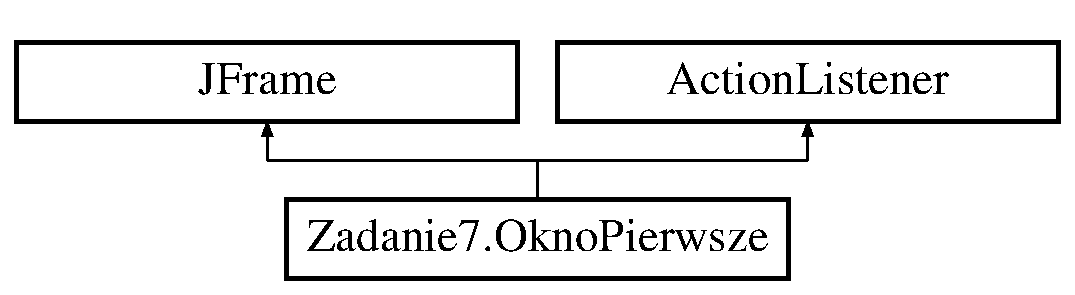
\includegraphics[height=2.000000cm]{class_zadanie7_1_1_okno_pierwsze}
\end{center}
\end{figure}
\subsection*{Public Member Functions}
\begin{DoxyCompactItemize}
\item 
\hyperlink{class_zadanie7_1_1_okno_pierwsze_aa4688831adc252f51059082333d5d487}{Okno\+Pierwsze} ()
\item 
void \hyperlink{class_zadanie7_1_1_okno_pierwsze_a2e3ea026f54071b2ed6c455a03913f60}{action\+Performed} (Action\+Event e)
\end{DoxyCompactItemize}
\subsection*{Package Attributes}
\begin{DoxyCompactItemize}
\item 
J\+Button \hyperlink{class_zadanie7_1_1_okno_pierwsze_aab4f419a650d2c8e5de90fc5eb75fc2b}{b1}
\item 
J\+Button \hyperlink{class_zadanie7_1_1_okno_pierwsze_a68b3a8081f2dedec7781e0908e4f8097}{b2}
\item 
J\+Label \hyperlink{class_zadanie7_1_1_okno_pierwsze_a63d3c938296a4de6303082d443a1a4e8}{l1}
\item 
J\+Label \hyperlink{class_zadanie7_1_1_okno_pierwsze_acb7e2e97fa47e9fbf8766edb58ea955b}{l2}
\item 
J\+Label \hyperlink{class_zadanie7_1_1_okno_pierwsze_ad23ac88cadae6e42871783c670d4ac02}{l3}
\item 
J\+Label \hyperlink{class_zadanie7_1_1_okno_pierwsze_adaa1ed1d82045750e6876c334a270a07}{l4}
\item 
J\+Text\+Field \hyperlink{class_zadanie7_1_1_okno_pierwsze_aa647d95695a358010c1c2d7801d2d3e0}{t1}
\item 
J\+Text\+Field \hyperlink{class_zadanie7_1_1_okno_pierwsze_a1a34a46dac7d3710c9abee8c74d52ef2}{t2}
\item 
J\+Text\+Field \hyperlink{class_zadanie7_1_1_okno_pierwsze_a7ab2f446b910b4a42d04e6d43dcbfc72}{t3}
\item 
J\+Text\+Field \hyperlink{class_zadanie7_1_1_okno_pierwsze_a23c1fb6015afadc86ce249d59d2d9543}{t4}
\end{DoxyCompactItemize}
\subsection*{Private Attributes}
\begin{DoxyCompactItemize}
\item 
int \hyperlink{class_zadanie7_1_1_okno_pierwsze_a8166de2f991b42c6eeebab44994e4305}{m}
\begin{DoxyCompactList}\small\item\em m-\/szerokosc \end{DoxyCompactList}\item 
int \hyperlink{class_zadanie7_1_1_okno_pierwsze_a4288fe2e8591c765e47e1396ee3ced8b}{n}
\begin{DoxyCompactList}\small\item\em n-\/wysokosc \end{DoxyCompactList}\item 
int \hyperlink{class_zadanie7_1_1_okno_pierwsze_a8f557e11c9083055333d31756f24e947}{p}
\begin{DoxyCompactList}\small\item\em p-\/prawdopodobienstwo \end{DoxyCompactList}\item 
int \hyperlink{class_zadanie7_1_1_okno_pierwsze_a90bcf5ebef62537bc74e27078a4f994b}{k}
\begin{DoxyCompactList}\small\item\em k-\/szybkosc \end{DoxyCompactList}\end{DoxyCompactItemize}
\subsection*{Static Private Attributes}
\begin{DoxyCompactItemize}
\item 
static final long \hyperlink{class_zadanie7_1_1_okno_pierwsze_ae27befaff5c47b70ff18a4e7ef92f4e0}{serial\+Version\+U\+ID} = 1L
\end{DoxyCompactItemize}


\subsection{Detailed Description}
\begin{DoxyAuthor}{Author}
Tymoteusz Surynt 
\end{DoxyAuthor}
\begin{DoxyVersion}{Version}
1.\+0 
\end{DoxyVersion}


\subsection{Constructor \& Destructor Documentation}
\index{Zadanie7\+::\+Okno\+Pierwsze@{Zadanie7\+::\+Okno\+Pierwsze}!Okno\+Pierwsze@{Okno\+Pierwsze}}
\index{Okno\+Pierwsze@{Okno\+Pierwsze}!Zadanie7\+::\+Okno\+Pierwsze@{Zadanie7\+::\+Okno\+Pierwsze}}
\subsubsection[{\texorpdfstring{Okno\+Pierwsze()}{OknoPierwsze()}}]{\setlength{\rightskip}{0pt plus 5cm}Zadanie7.\+Okno\+Pierwsze.\+Okno\+Pierwsze (
\begin{DoxyParamCaption}
{}
\end{DoxyParamCaption}
)}\hypertarget{class_zadanie7_1_1_okno_pierwsze_aa4688831adc252f51059082333d5d487}{}\label{class_zadanie7_1_1_okno_pierwsze_aa4688831adc252f51059082333d5d487}


\subsection{Member Function Documentation}
\index{Zadanie7\+::\+Okno\+Pierwsze@{Zadanie7\+::\+Okno\+Pierwsze}!action\+Performed@{action\+Performed}}
\index{action\+Performed@{action\+Performed}!Zadanie7\+::\+Okno\+Pierwsze@{Zadanie7\+::\+Okno\+Pierwsze}}
\subsubsection[{\texorpdfstring{action\+Performed(\+Action\+Event e)}{actionPerformed(ActionEvent e)}}]{\setlength{\rightskip}{0pt plus 5cm}void Zadanie7.\+Okno\+Pierwsze.\+action\+Performed (
\begin{DoxyParamCaption}
\item[{Action\+Event}]{e}
\end{DoxyParamCaption}
)}\hypertarget{class_zadanie7_1_1_okno_pierwsze_a2e3ea026f54071b2ed6c455a03913f60}{}\label{class_zadanie7_1_1_okno_pierwsze_a2e3ea026f54071b2ed6c455a03913f60}


\subsection{Member Data Documentation}
\index{Zadanie7\+::\+Okno\+Pierwsze@{Zadanie7\+::\+Okno\+Pierwsze}!b1@{b1}}
\index{b1@{b1}!Zadanie7\+::\+Okno\+Pierwsze@{Zadanie7\+::\+Okno\+Pierwsze}}
\subsubsection[{\texorpdfstring{b1}{b1}}]{\setlength{\rightskip}{0pt plus 5cm}J\+Button Zadanie7.\+Okno\+Pierwsze.\+b1\hspace{0.3cm}{\ttfamily [package]}}\hypertarget{class_zadanie7_1_1_okno_pierwsze_aab4f419a650d2c8e5de90fc5eb75fc2b}{}\label{class_zadanie7_1_1_okno_pierwsze_aab4f419a650d2c8e5de90fc5eb75fc2b}
\index{Zadanie7\+::\+Okno\+Pierwsze@{Zadanie7\+::\+Okno\+Pierwsze}!b2@{b2}}
\index{b2@{b2}!Zadanie7\+::\+Okno\+Pierwsze@{Zadanie7\+::\+Okno\+Pierwsze}}
\subsubsection[{\texorpdfstring{b2}{b2}}]{\setlength{\rightskip}{0pt plus 5cm}J\+Button Zadanie7.\+Okno\+Pierwsze.\+b2\hspace{0.3cm}{\ttfamily [package]}}\hypertarget{class_zadanie7_1_1_okno_pierwsze_a68b3a8081f2dedec7781e0908e4f8097}{}\label{class_zadanie7_1_1_okno_pierwsze_a68b3a8081f2dedec7781e0908e4f8097}
\index{Zadanie7\+::\+Okno\+Pierwsze@{Zadanie7\+::\+Okno\+Pierwsze}!k@{k}}
\index{k@{k}!Zadanie7\+::\+Okno\+Pierwsze@{Zadanie7\+::\+Okno\+Pierwsze}}
\subsubsection[{\texorpdfstring{k}{k}}]{\setlength{\rightskip}{0pt plus 5cm}int Zadanie7.\+Okno\+Pierwsze.\+k\hspace{0.3cm}{\ttfamily [private]}}\hypertarget{class_zadanie7_1_1_okno_pierwsze_a90bcf5ebef62537bc74e27078a4f994b}{}\label{class_zadanie7_1_1_okno_pierwsze_a90bcf5ebef62537bc74e27078a4f994b}


k-\/szybkosc 

\index{Zadanie7\+::\+Okno\+Pierwsze@{Zadanie7\+::\+Okno\+Pierwsze}!l1@{l1}}
\index{l1@{l1}!Zadanie7\+::\+Okno\+Pierwsze@{Zadanie7\+::\+Okno\+Pierwsze}}
\subsubsection[{\texorpdfstring{l1}{l1}}]{\setlength{\rightskip}{0pt plus 5cm}J\+Label Zadanie7.\+Okno\+Pierwsze.\+l1\hspace{0.3cm}{\ttfamily [package]}}\hypertarget{class_zadanie7_1_1_okno_pierwsze_a63d3c938296a4de6303082d443a1a4e8}{}\label{class_zadanie7_1_1_okno_pierwsze_a63d3c938296a4de6303082d443a1a4e8}
\index{Zadanie7\+::\+Okno\+Pierwsze@{Zadanie7\+::\+Okno\+Pierwsze}!l2@{l2}}
\index{l2@{l2}!Zadanie7\+::\+Okno\+Pierwsze@{Zadanie7\+::\+Okno\+Pierwsze}}
\subsubsection[{\texorpdfstring{l2}{l2}}]{\setlength{\rightskip}{0pt plus 5cm}J\+Label Zadanie7.\+Okno\+Pierwsze.\+l2\hspace{0.3cm}{\ttfamily [package]}}\hypertarget{class_zadanie7_1_1_okno_pierwsze_acb7e2e97fa47e9fbf8766edb58ea955b}{}\label{class_zadanie7_1_1_okno_pierwsze_acb7e2e97fa47e9fbf8766edb58ea955b}
\index{Zadanie7\+::\+Okno\+Pierwsze@{Zadanie7\+::\+Okno\+Pierwsze}!l3@{l3}}
\index{l3@{l3}!Zadanie7\+::\+Okno\+Pierwsze@{Zadanie7\+::\+Okno\+Pierwsze}}
\subsubsection[{\texorpdfstring{l3}{l3}}]{\setlength{\rightskip}{0pt plus 5cm}J\+Label Zadanie7.\+Okno\+Pierwsze.\+l3\hspace{0.3cm}{\ttfamily [package]}}\hypertarget{class_zadanie7_1_1_okno_pierwsze_ad23ac88cadae6e42871783c670d4ac02}{}\label{class_zadanie7_1_1_okno_pierwsze_ad23ac88cadae6e42871783c670d4ac02}
\index{Zadanie7\+::\+Okno\+Pierwsze@{Zadanie7\+::\+Okno\+Pierwsze}!l4@{l4}}
\index{l4@{l4}!Zadanie7\+::\+Okno\+Pierwsze@{Zadanie7\+::\+Okno\+Pierwsze}}
\subsubsection[{\texorpdfstring{l4}{l4}}]{\setlength{\rightskip}{0pt plus 5cm}J\+Label Zadanie7.\+Okno\+Pierwsze.\+l4\hspace{0.3cm}{\ttfamily [package]}}\hypertarget{class_zadanie7_1_1_okno_pierwsze_adaa1ed1d82045750e6876c334a270a07}{}\label{class_zadanie7_1_1_okno_pierwsze_adaa1ed1d82045750e6876c334a270a07}
\index{Zadanie7\+::\+Okno\+Pierwsze@{Zadanie7\+::\+Okno\+Pierwsze}!m@{m}}
\index{m@{m}!Zadanie7\+::\+Okno\+Pierwsze@{Zadanie7\+::\+Okno\+Pierwsze}}
\subsubsection[{\texorpdfstring{m}{m}}]{\setlength{\rightskip}{0pt plus 5cm}int Zadanie7.\+Okno\+Pierwsze.\+m\hspace{0.3cm}{\ttfamily [private]}}\hypertarget{class_zadanie7_1_1_okno_pierwsze_a8166de2f991b42c6eeebab44994e4305}{}\label{class_zadanie7_1_1_okno_pierwsze_a8166de2f991b42c6eeebab44994e4305}


m-\/szerokosc 

\index{Zadanie7\+::\+Okno\+Pierwsze@{Zadanie7\+::\+Okno\+Pierwsze}!n@{n}}
\index{n@{n}!Zadanie7\+::\+Okno\+Pierwsze@{Zadanie7\+::\+Okno\+Pierwsze}}
\subsubsection[{\texorpdfstring{n}{n}}]{\setlength{\rightskip}{0pt plus 5cm}int Zadanie7.\+Okno\+Pierwsze.\+n\hspace{0.3cm}{\ttfamily [private]}}\hypertarget{class_zadanie7_1_1_okno_pierwsze_a4288fe2e8591c765e47e1396ee3ced8b}{}\label{class_zadanie7_1_1_okno_pierwsze_a4288fe2e8591c765e47e1396ee3ced8b}


n-\/wysokosc 

\index{Zadanie7\+::\+Okno\+Pierwsze@{Zadanie7\+::\+Okno\+Pierwsze}!p@{p}}
\index{p@{p}!Zadanie7\+::\+Okno\+Pierwsze@{Zadanie7\+::\+Okno\+Pierwsze}}
\subsubsection[{\texorpdfstring{p}{p}}]{\setlength{\rightskip}{0pt plus 5cm}int Zadanie7.\+Okno\+Pierwsze.\+p\hspace{0.3cm}{\ttfamily [private]}}\hypertarget{class_zadanie7_1_1_okno_pierwsze_a8f557e11c9083055333d31756f24e947}{}\label{class_zadanie7_1_1_okno_pierwsze_a8f557e11c9083055333d31756f24e947}


p-\/prawdopodobienstwo 

\index{Zadanie7\+::\+Okno\+Pierwsze@{Zadanie7\+::\+Okno\+Pierwsze}!serial\+Version\+U\+ID@{serial\+Version\+U\+ID}}
\index{serial\+Version\+U\+ID@{serial\+Version\+U\+ID}!Zadanie7\+::\+Okno\+Pierwsze@{Zadanie7\+::\+Okno\+Pierwsze}}
\subsubsection[{\texorpdfstring{serial\+Version\+U\+ID}{serialVersionUID}}]{\setlength{\rightskip}{0pt plus 5cm}final long Zadanie7.\+Okno\+Pierwsze.\+serial\+Version\+U\+ID = 1L\hspace{0.3cm}{\ttfamily [static]}, {\ttfamily [private]}}\hypertarget{class_zadanie7_1_1_okno_pierwsze_ae27befaff5c47b70ff18a4e7ef92f4e0}{}\label{class_zadanie7_1_1_okno_pierwsze_ae27befaff5c47b70ff18a4e7ef92f4e0}
\index{Zadanie7\+::\+Okno\+Pierwsze@{Zadanie7\+::\+Okno\+Pierwsze}!t1@{t1}}
\index{t1@{t1}!Zadanie7\+::\+Okno\+Pierwsze@{Zadanie7\+::\+Okno\+Pierwsze}}
\subsubsection[{\texorpdfstring{t1}{t1}}]{\setlength{\rightskip}{0pt plus 5cm}J\+Text\+Field Zadanie7.\+Okno\+Pierwsze.\+t1\hspace{0.3cm}{\ttfamily [package]}}\hypertarget{class_zadanie7_1_1_okno_pierwsze_aa647d95695a358010c1c2d7801d2d3e0}{}\label{class_zadanie7_1_1_okno_pierwsze_aa647d95695a358010c1c2d7801d2d3e0}
\index{Zadanie7\+::\+Okno\+Pierwsze@{Zadanie7\+::\+Okno\+Pierwsze}!t2@{t2}}
\index{t2@{t2}!Zadanie7\+::\+Okno\+Pierwsze@{Zadanie7\+::\+Okno\+Pierwsze}}
\subsubsection[{\texorpdfstring{t2}{t2}}]{\setlength{\rightskip}{0pt plus 5cm}J\+Text\+Field Zadanie7.\+Okno\+Pierwsze.\+t2\hspace{0.3cm}{\ttfamily [package]}}\hypertarget{class_zadanie7_1_1_okno_pierwsze_a1a34a46dac7d3710c9abee8c74d52ef2}{}\label{class_zadanie7_1_1_okno_pierwsze_a1a34a46dac7d3710c9abee8c74d52ef2}
\index{Zadanie7\+::\+Okno\+Pierwsze@{Zadanie7\+::\+Okno\+Pierwsze}!t3@{t3}}
\index{t3@{t3}!Zadanie7\+::\+Okno\+Pierwsze@{Zadanie7\+::\+Okno\+Pierwsze}}
\subsubsection[{\texorpdfstring{t3}{t3}}]{\setlength{\rightskip}{0pt plus 5cm}J\+Text\+Field Zadanie7.\+Okno\+Pierwsze.\+t3\hspace{0.3cm}{\ttfamily [package]}}\hypertarget{class_zadanie7_1_1_okno_pierwsze_a7ab2f446b910b4a42d04e6d43dcbfc72}{}\label{class_zadanie7_1_1_okno_pierwsze_a7ab2f446b910b4a42d04e6d43dcbfc72}
\index{Zadanie7\+::\+Okno\+Pierwsze@{Zadanie7\+::\+Okno\+Pierwsze}!t4@{t4}}
\index{t4@{t4}!Zadanie7\+::\+Okno\+Pierwsze@{Zadanie7\+::\+Okno\+Pierwsze}}
\subsubsection[{\texorpdfstring{t4}{t4}}]{\setlength{\rightskip}{0pt plus 5cm}J\+Text\+Field Zadanie7.\+Okno\+Pierwsze.\+t4\hspace{0.3cm}{\ttfamily [package]}}\hypertarget{class_zadanie7_1_1_okno_pierwsze_a23c1fb6015afadc86ce249d59d2d9543}{}\label{class_zadanie7_1_1_okno_pierwsze_a23c1fb6015afadc86ce249d59d2d9543}


The documentation for this class was generated from the following file\+:\begin{DoxyCompactItemize}
\item 
\hyperlink{_okno_pierwsze_8java}{Okno\+Pierwsze.\+java}\end{DoxyCompactItemize}

\hypertarget{class_zadanie7_1_1_okno_wlasciwe}{}\section{Zadanie7.\+Okno\+Wlasciwe Class Reference}
\label{class_zadanie7_1_1_okno_wlasciwe}\index{Zadanie7.\+Okno\+Wlasciwe@{Zadanie7.\+Okno\+Wlasciwe}}
Inheritance diagram for Zadanie7.\+Okno\+Wlasciwe\+:\begin{figure}[H]
\begin{center}
\leavevmode
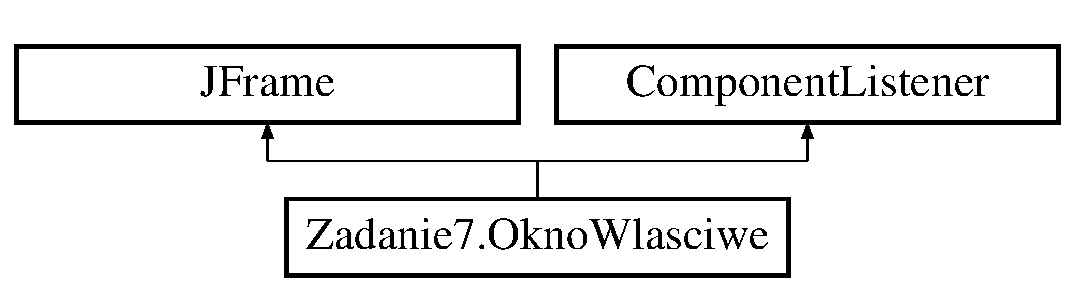
\includegraphics[height=2.000000cm]{class_zadanie7_1_1_okno_wlasciwe}
\end{center}
\end{figure}
\subsection*{Classes}
\begin{DoxyCompactItemize}
\item 
class \hyperlink{class_zadanie7_1_1_okno_wlasciwe_1_1_watki_wlasciwe}{Watki\+Wlasciwe}
\end{DoxyCompactItemize}
\subsection*{Public Member Functions}
\begin{DoxyCompactItemize}
\item 
void \hyperlink{class_zadanie7_1_1_okno_wlasciwe_ad6be5bc65e9c28156611abe622b27fd6}{paint} (Graphics g)
\begin{DoxyCompactList}\small\item\em podwojne buforowanie \end{DoxyCompactList}\item 
void \hyperlink{class_zadanie7_1_1_okno_wlasciwe_a2cfd87352800ef1a9aa7746033a5436b}{paint\+Components} (Graphics g)
\begin{DoxyCompactList}\small\item\em rysowanie boksow \end{DoxyCompactList}\item 
void \hyperlink{class_zadanie7_1_1_okno_wlasciwe_a48ca8c4ab5ec7949801e31a2359a689f}{component\+Resized} (Component\+Event e)
\begin{DoxyCompactList}\small\item\em skalowanie, zaleznie od wielkosci nowego okna \end{DoxyCompactList}\item 
void \hyperlink{class_zadanie7_1_1_okno_wlasciwe_a5691cd056cd2bf85af4f53e29fed7b43}{component\+Hidden} (Component\+Event arg0)
\item 
void \hyperlink{class_zadanie7_1_1_okno_wlasciwe_a64d00ee7a3be96cfabb548ee54fe7915}{component\+Moved} (Component\+Event arg0)
\item 
void \hyperlink{class_zadanie7_1_1_okno_wlasciwe_ab2ee70e1ec0517025b4530f963321dd4}{component\+Shown} (Component\+Event arg0)
\end{DoxyCompactItemize}
\subsection*{Package Functions}
\begin{DoxyCompactItemize}
\item 
\hyperlink{class_zadanie7_1_1_okno_wlasciwe_a09f8c68cad5eb49f7229c1141acfd832}{Okno\+Wlasciwe} (int \hyperlink{class_zadanie7_1_1_okno_wlasciwe_a2ac6a5aa6284f4835a12a68754ae80b8}{m}, int \hyperlink{class_zadanie7_1_1_okno_wlasciwe_a9def326ff03537e3e304e17fc99ab674}{n}, int k, int p)
\begin{DoxyCompactList}\small\item\em Generowanie planszy z symulacja. \end{DoxyCompactList}\end{DoxyCompactItemize}
\subsection*{Private Attributes}
\begin{DoxyCompactItemize}
\item 
Random \hyperlink{class_zadanie7_1_1_okno_wlasciwe_a9ae176d92e991a053b101aad6fdf7cdf}{los} =new Random()
\begin{DoxyCompactList}\small\item\em los-\/jedyny generator losowy \end{DoxyCompactList}\item 
double \hyperlink{class_zadanie7_1_1_okno_wlasciwe_afc22e58c9c97b94e580568fb79a36bef}{x} =20
\begin{DoxyCompactList}\small\item\em x-\/wspolrzedna x, przesunieta o 20 w celu otrzymania lepszego efektu graficznego \end{DoxyCompactList}\item 
double \hyperlink{class_zadanie7_1_1_okno_wlasciwe_a59d4e6fb76e7711fb07bfcb0df74d9e6}{y} =40
\begin{DoxyCompactList}\small\item\em y-\/wspolrzedna y, przesunieta o 40 w celu otrzymania lepszego efektu graficznego \end{DoxyCompactList}\item 
double \hyperlink{class_zadanie7_1_1_okno_wlasciwe_a160d088398a77a3897d8bac099c56577}{w}
\begin{DoxyCompactList}\small\item\em w-\/szerokosc naszego boksu \end{DoxyCompactList}\item 
double \hyperlink{class_zadanie7_1_1_okno_wlasciwe_ac8bed36b0724579fa1bab6098bbd4204}{h}
\begin{DoxyCompactList}\small\item\em h-\/wysokosc naszego boksu \end{DoxyCompactList}\item 
int \hyperlink{class_zadanie7_1_1_okno_wlasciwe_a2ac6a5aa6284f4835a12a68754ae80b8}{m}
\begin{DoxyCompactList}\small\item\em szerokosc planszy liczona w boksach \end{DoxyCompactList}\item 
int \hyperlink{class_zadanie7_1_1_okno_wlasciwe_a9def326ff03537e3e304e17fc99ab674}{n}
\begin{DoxyCompactList}\small\item\em wysokosc planszy liczona w boksach \end{DoxyCompactList}\item 
Rectangle2D\mbox{[}$\,$\mbox{]}\mbox{[}$\,$\mbox{]} \hyperlink{class_zadanie7_1_1_okno_wlasciwe_a76e7cdaa5f7d262c3466f9e28126a1a4}{t}
\begin{DoxyCompactList}\small\item\em t-\/ tablica prostokatow ktore beda robic za boksy \end{DoxyCompactList}\item 
Color\mbox{[}$\,$\mbox{]}\mbox{[}$\,$\mbox{]} \hyperlink{class_zadanie7_1_1_okno_wlasciwe_a6adcf3f4cbee43c70583647ed34b9db4}{kolor}
\begin{DoxyCompactList}\small\item\em kolor-\/ tablica kolorow \end{DoxyCompactList}\item 
\hyperlink{class_zadanie7_1_1_okno_wlasciwe_1_1_watki_wlasciwe}{Watki\+Wlasciwe}\mbox{[}$\,$\mbox{]}\mbox{[}$\,$\mbox{]} \hyperlink{class_zadanie7_1_1_okno_wlasciwe_ac767c1f94c8102a043d4cd4f85eb99ba}{a}
\begin{DoxyCompactList}\small\item\em a-\/tablica watkow \end{DoxyCompactList}\item 
Image \hyperlink{class_zadanie7_1_1_okno_wlasciwe_acb927a7852ab3d56d14b896ccbac3446}{obraz}
\item 
Graphics \hyperlink{class_zadanie7_1_1_okno_wlasciwe_ae40d1f4b0ba77778e9aff178a22d8caf}{g22}
\end{DoxyCompactItemize}
\subsection*{Static Private Attributes}
\begin{DoxyCompactItemize}
\item 
static final long \hyperlink{class_zadanie7_1_1_okno_wlasciwe_ad82a67e6a62aab90682d92db18f794d1}{serial\+Version\+U\+ID} = 1L
\end{DoxyCompactItemize}


\subsection{Detailed Description}
\begin{DoxyAuthor}{Author}
Tymoteusz Surynt 
\end{DoxyAuthor}
\begin{DoxyVersion}{Version}
1.\+0 
\end{DoxyVersion}


\subsection{Constructor \& Destructor Documentation}
\index{Zadanie7\+::\+Okno\+Wlasciwe@{Zadanie7\+::\+Okno\+Wlasciwe}!Okno\+Wlasciwe@{Okno\+Wlasciwe}}
\index{Okno\+Wlasciwe@{Okno\+Wlasciwe}!Zadanie7\+::\+Okno\+Wlasciwe@{Zadanie7\+::\+Okno\+Wlasciwe}}
\subsubsection[{\texorpdfstring{Okno\+Wlasciwe(int m, int n, int k, int p)}{OknoWlasciwe(int m, int n, int k, int p)}}]{\setlength{\rightskip}{0pt plus 5cm}Zadanie7.\+Okno\+Wlasciwe.\+Okno\+Wlasciwe (
\begin{DoxyParamCaption}
\item[{int}]{m, }
\item[{int}]{n, }
\item[{int}]{k, }
\item[{int}]{p}
\end{DoxyParamCaption}
)\hspace{0.3cm}{\ttfamily [package]}}\hypertarget{class_zadanie7_1_1_okno_wlasciwe_a09f8c68cad5eb49f7229c1141acfd832}{}\label{class_zadanie7_1_1_okno_wlasciwe_a09f8c68cad5eb49f7229c1141acfd832}


Generowanie planszy z symulacja. 


\begin{DoxyParams}{Parameters}
{\em m} & szerokosc planszy liczona w boksach (int) \\
\hline
{\em n} & wysokosc planszy liczona w boksach (int) \\
\hline
{\em k} & szybkosc dzialania programu, im wiecej tym wolniej (int) \\
\hline
{\em p} & prawdopodobienstwo w procentach (int) \\
\hline
\end{DoxyParams}


\subsection{Member Function Documentation}
\index{Zadanie7\+::\+Okno\+Wlasciwe@{Zadanie7\+::\+Okno\+Wlasciwe}!component\+Hidden@{component\+Hidden}}
\index{component\+Hidden@{component\+Hidden}!Zadanie7\+::\+Okno\+Wlasciwe@{Zadanie7\+::\+Okno\+Wlasciwe}}
\subsubsection[{\texorpdfstring{component\+Hidden(\+Component\+Event arg0)}{componentHidden(ComponentEvent arg0)}}]{\setlength{\rightskip}{0pt plus 5cm}void Zadanie7.\+Okno\+Wlasciwe.\+component\+Hidden (
\begin{DoxyParamCaption}
\item[{Component\+Event}]{arg0}
\end{DoxyParamCaption}
)}\hypertarget{class_zadanie7_1_1_okno_wlasciwe_a5691cd056cd2bf85af4f53e29fed7b43}{}\label{class_zadanie7_1_1_okno_wlasciwe_a5691cd056cd2bf85af4f53e29fed7b43}
\index{Zadanie7\+::\+Okno\+Wlasciwe@{Zadanie7\+::\+Okno\+Wlasciwe}!component\+Moved@{component\+Moved}}
\index{component\+Moved@{component\+Moved}!Zadanie7\+::\+Okno\+Wlasciwe@{Zadanie7\+::\+Okno\+Wlasciwe}}
\subsubsection[{\texorpdfstring{component\+Moved(\+Component\+Event arg0)}{componentMoved(ComponentEvent arg0)}}]{\setlength{\rightskip}{0pt plus 5cm}void Zadanie7.\+Okno\+Wlasciwe.\+component\+Moved (
\begin{DoxyParamCaption}
\item[{Component\+Event}]{arg0}
\end{DoxyParamCaption}
)}\hypertarget{class_zadanie7_1_1_okno_wlasciwe_a64d00ee7a3be96cfabb548ee54fe7915}{}\label{class_zadanie7_1_1_okno_wlasciwe_a64d00ee7a3be96cfabb548ee54fe7915}
\index{Zadanie7\+::\+Okno\+Wlasciwe@{Zadanie7\+::\+Okno\+Wlasciwe}!component\+Resized@{component\+Resized}}
\index{component\+Resized@{component\+Resized}!Zadanie7\+::\+Okno\+Wlasciwe@{Zadanie7\+::\+Okno\+Wlasciwe}}
\subsubsection[{\texorpdfstring{component\+Resized(\+Component\+Event e)}{componentResized(ComponentEvent e)}}]{\setlength{\rightskip}{0pt plus 5cm}void Zadanie7.\+Okno\+Wlasciwe.\+component\+Resized (
\begin{DoxyParamCaption}
\item[{Component\+Event}]{e}
\end{DoxyParamCaption}
)}\hypertarget{class_zadanie7_1_1_okno_wlasciwe_a48ca8c4ab5ec7949801e31a2359a689f}{}\label{class_zadanie7_1_1_okno_wlasciwe_a48ca8c4ab5ec7949801e31a2359a689f}


skalowanie, zaleznie od wielkosci nowego okna 

\index{Zadanie7\+::\+Okno\+Wlasciwe@{Zadanie7\+::\+Okno\+Wlasciwe}!component\+Shown@{component\+Shown}}
\index{component\+Shown@{component\+Shown}!Zadanie7\+::\+Okno\+Wlasciwe@{Zadanie7\+::\+Okno\+Wlasciwe}}
\subsubsection[{\texorpdfstring{component\+Shown(\+Component\+Event arg0)}{componentShown(ComponentEvent arg0)}}]{\setlength{\rightskip}{0pt plus 5cm}void Zadanie7.\+Okno\+Wlasciwe.\+component\+Shown (
\begin{DoxyParamCaption}
\item[{Component\+Event}]{arg0}
\end{DoxyParamCaption}
)}\hypertarget{class_zadanie7_1_1_okno_wlasciwe_ab2ee70e1ec0517025b4530f963321dd4}{}\label{class_zadanie7_1_1_okno_wlasciwe_ab2ee70e1ec0517025b4530f963321dd4}
\index{Zadanie7\+::\+Okno\+Wlasciwe@{Zadanie7\+::\+Okno\+Wlasciwe}!paint@{paint}}
\index{paint@{paint}!Zadanie7\+::\+Okno\+Wlasciwe@{Zadanie7\+::\+Okno\+Wlasciwe}}
\subsubsection[{\texorpdfstring{paint(\+Graphics g)}{paint(Graphics g)}}]{\setlength{\rightskip}{0pt plus 5cm}void Zadanie7.\+Okno\+Wlasciwe.\+paint (
\begin{DoxyParamCaption}
\item[{Graphics}]{g}
\end{DoxyParamCaption}
)}\hypertarget{class_zadanie7_1_1_okno_wlasciwe_ad6be5bc65e9c28156611abe622b27fd6}{}\label{class_zadanie7_1_1_okno_wlasciwe_ad6be5bc65e9c28156611abe622b27fd6}


podwojne buforowanie 

\index{Zadanie7\+::\+Okno\+Wlasciwe@{Zadanie7\+::\+Okno\+Wlasciwe}!paint\+Components@{paint\+Components}}
\index{paint\+Components@{paint\+Components}!Zadanie7\+::\+Okno\+Wlasciwe@{Zadanie7\+::\+Okno\+Wlasciwe}}
\subsubsection[{\texorpdfstring{paint\+Components(\+Graphics g)}{paintComponents(Graphics g)}}]{\setlength{\rightskip}{0pt plus 5cm}void Zadanie7.\+Okno\+Wlasciwe.\+paint\+Components (
\begin{DoxyParamCaption}
\item[{Graphics}]{g}
\end{DoxyParamCaption}
)}\hypertarget{class_zadanie7_1_1_okno_wlasciwe_a2cfd87352800ef1a9aa7746033a5436b}{}\label{class_zadanie7_1_1_okno_wlasciwe_a2cfd87352800ef1a9aa7746033a5436b}


rysowanie boksow 



\subsection{Member Data Documentation}
\index{Zadanie7\+::\+Okno\+Wlasciwe@{Zadanie7\+::\+Okno\+Wlasciwe}!a@{a}}
\index{a@{a}!Zadanie7\+::\+Okno\+Wlasciwe@{Zadanie7\+::\+Okno\+Wlasciwe}}
\subsubsection[{\texorpdfstring{a}{a}}]{\setlength{\rightskip}{0pt plus 5cm}{\bf Watki\+Wlasciwe} \mbox{[}$\,$\mbox{]}\mbox{[}$\,$\mbox{]} Zadanie7.\+Okno\+Wlasciwe.\+a\hspace{0.3cm}{\ttfamily [private]}}\hypertarget{class_zadanie7_1_1_okno_wlasciwe_ac767c1f94c8102a043d4cd4f85eb99ba}{}\label{class_zadanie7_1_1_okno_wlasciwe_ac767c1f94c8102a043d4cd4f85eb99ba}


a-\/tablica watkow 

\index{Zadanie7\+::\+Okno\+Wlasciwe@{Zadanie7\+::\+Okno\+Wlasciwe}!g22@{g22}}
\index{g22@{g22}!Zadanie7\+::\+Okno\+Wlasciwe@{Zadanie7\+::\+Okno\+Wlasciwe}}
\subsubsection[{\texorpdfstring{g22}{g22}}]{\setlength{\rightskip}{0pt plus 5cm}Graphics Zadanie7.\+Okno\+Wlasciwe.\+g22\hspace{0.3cm}{\ttfamily [private]}}\hypertarget{class_zadanie7_1_1_okno_wlasciwe_ae40d1f4b0ba77778e9aff178a22d8caf}{}\label{class_zadanie7_1_1_okno_wlasciwe_ae40d1f4b0ba77778e9aff178a22d8caf}
\index{Zadanie7\+::\+Okno\+Wlasciwe@{Zadanie7\+::\+Okno\+Wlasciwe}!h@{h}}
\index{h@{h}!Zadanie7\+::\+Okno\+Wlasciwe@{Zadanie7\+::\+Okno\+Wlasciwe}}
\subsubsection[{\texorpdfstring{h}{h}}]{\setlength{\rightskip}{0pt plus 5cm}double Zadanie7.\+Okno\+Wlasciwe.\+h\hspace{0.3cm}{\ttfamily [private]}}\hypertarget{class_zadanie7_1_1_okno_wlasciwe_ac8bed36b0724579fa1bab6098bbd4204}{}\label{class_zadanie7_1_1_okno_wlasciwe_ac8bed36b0724579fa1bab6098bbd4204}


h-\/wysokosc naszego boksu 

\index{Zadanie7\+::\+Okno\+Wlasciwe@{Zadanie7\+::\+Okno\+Wlasciwe}!kolor@{kolor}}
\index{kolor@{kolor}!Zadanie7\+::\+Okno\+Wlasciwe@{Zadanie7\+::\+Okno\+Wlasciwe}}
\subsubsection[{\texorpdfstring{kolor}{kolor}}]{\setlength{\rightskip}{0pt plus 5cm}Color \mbox{[}$\,$\mbox{]}\mbox{[}$\,$\mbox{]} Zadanie7.\+Okno\+Wlasciwe.\+kolor\hspace{0.3cm}{\ttfamily [private]}}\hypertarget{class_zadanie7_1_1_okno_wlasciwe_a6adcf3f4cbee43c70583647ed34b9db4}{}\label{class_zadanie7_1_1_okno_wlasciwe_a6adcf3f4cbee43c70583647ed34b9db4}


kolor-\/ tablica kolorow 

\index{Zadanie7\+::\+Okno\+Wlasciwe@{Zadanie7\+::\+Okno\+Wlasciwe}!los@{los}}
\index{los@{los}!Zadanie7\+::\+Okno\+Wlasciwe@{Zadanie7\+::\+Okno\+Wlasciwe}}
\subsubsection[{\texorpdfstring{los}{los}}]{\setlength{\rightskip}{0pt plus 5cm}Random Zadanie7.\+Okno\+Wlasciwe.\+los =new Random()\hspace{0.3cm}{\ttfamily [private]}}\hypertarget{class_zadanie7_1_1_okno_wlasciwe_a9ae176d92e991a053b101aad6fdf7cdf}{}\label{class_zadanie7_1_1_okno_wlasciwe_a9ae176d92e991a053b101aad6fdf7cdf}


los-\/jedyny generator losowy 

\index{Zadanie7\+::\+Okno\+Wlasciwe@{Zadanie7\+::\+Okno\+Wlasciwe}!m@{m}}
\index{m@{m}!Zadanie7\+::\+Okno\+Wlasciwe@{Zadanie7\+::\+Okno\+Wlasciwe}}
\subsubsection[{\texorpdfstring{m}{m}}]{\setlength{\rightskip}{0pt plus 5cm}int Zadanie7.\+Okno\+Wlasciwe.\+m\hspace{0.3cm}{\ttfamily [private]}}\hypertarget{class_zadanie7_1_1_okno_wlasciwe_a2ac6a5aa6284f4835a12a68754ae80b8}{}\label{class_zadanie7_1_1_okno_wlasciwe_a2ac6a5aa6284f4835a12a68754ae80b8}


szerokosc planszy liczona w boksach 

\begin{DoxySeeAlso}{See also}
\hyperlink{class_zadanie7_1_1_okno_pierwsze_a8166de2f991b42c6eeebab44994e4305}{Zadanie7.\+Okno\+Pierwsze\+::m} szerokosc 
\end{DoxySeeAlso}
\index{Zadanie7\+::\+Okno\+Wlasciwe@{Zadanie7\+::\+Okno\+Wlasciwe}!n@{n}}
\index{n@{n}!Zadanie7\+::\+Okno\+Wlasciwe@{Zadanie7\+::\+Okno\+Wlasciwe}}
\subsubsection[{\texorpdfstring{n}{n}}]{\setlength{\rightskip}{0pt plus 5cm}int Zadanie7.\+Okno\+Wlasciwe.\+n\hspace{0.3cm}{\ttfamily [private]}}\hypertarget{class_zadanie7_1_1_okno_wlasciwe_a9def326ff03537e3e304e17fc99ab674}{}\label{class_zadanie7_1_1_okno_wlasciwe_a9def326ff03537e3e304e17fc99ab674}


wysokosc planszy liczona w boksach 

\begin{DoxySeeAlso}{See also}
\hyperlink{class_zadanie7_1_1_okno_pierwsze_a4288fe2e8591c765e47e1396ee3ced8b}{Zadanie7.\+Okno\+Pierwsze\+::n} wysokosc 
\end{DoxySeeAlso}
\index{Zadanie7\+::\+Okno\+Wlasciwe@{Zadanie7\+::\+Okno\+Wlasciwe}!obraz@{obraz}}
\index{obraz@{obraz}!Zadanie7\+::\+Okno\+Wlasciwe@{Zadanie7\+::\+Okno\+Wlasciwe}}
\subsubsection[{\texorpdfstring{obraz}{obraz}}]{\setlength{\rightskip}{0pt plus 5cm}Image Zadanie7.\+Okno\+Wlasciwe.\+obraz\hspace{0.3cm}{\ttfamily [private]}}\hypertarget{class_zadanie7_1_1_okno_wlasciwe_acb927a7852ab3d56d14b896ccbac3446}{}\label{class_zadanie7_1_1_okno_wlasciwe_acb927a7852ab3d56d14b896ccbac3446}
\index{Zadanie7\+::\+Okno\+Wlasciwe@{Zadanie7\+::\+Okno\+Wlasciwe}!serial\+Version\+U\+ID@{serial\+Version\+U\+ID}}
\index{serial\+Version\+U\+ID@{serial\+Version\+U\+ID}!Zadanie7\+::\+Okno\+Wlasciwe@{Zadanie7\+::\+Okno\+Wlasciwe}}
\subsubsection[{\texorpdfstring{serial\+Version\+U\+ID}{serialVersionUID}}]{\setlength{\rightskip}{0pt plus 5cm}final long Zadanie7.\+Okno\+Wlasciwe.\+serial\+Version\+U\+ID = 1L\hspace{0.3cm}{\ttfamily [static]}, {\ttfamily [private]}}\hypertarget{class_zadanie7_1_1_okno_wlasciwe_ad82a67e6a62aab90682d92db18f794d1}{}\label{class_zadanie7_1_1_okno_wlasciwe_ad82a67e6a62aab90682d92db18f794d1}
\index{Zadanie7\+::\+Okno\+Wlasciwe@{Zadanie7\+::\+Okno\+Wlasciwe}!t@{t}}
\index{t@{t}!Zadanie7\+::\+Okno\+Wlasciwe@{Zadanie7\+::\+Okno\+Wlasciwe}}
\subsubsection[{\texorpdfstring{t}{t}}]{\setlength{\rightskip}{0pt plus 5cm}Rectangle2D \mbox{[}$\,$\mbox{]}\mbox{[}$\,$\mbox{]} Zadanie7.\+Okno\+Wlasciwe.\+t\hspace{0.3cm}{\ttfamily [private]}}\hypertarget{class_zadanie7_1_1_okno_wlasciwe_a76e7cdaa5f7d262c3466f9e28126a1a4}{}\label{class_zadanie7_1_1_okno_wlasciwe_a76e7cdaa5f7d262c3466f9e28126a1a4}


t-\/ tablica prostokatow ktore beda robic za boksy 

\index{Zadanie7\+::\+Okno\+Wlasciwe@{Zadanie7\+::\+Okno\+Wlasciwe}!w@{w}}
\index{w@{w}!Zadanie7\+::\+Okno\+Wlasciwe@{Zadanie7\+::\+Okno\+Wlasciwe}}
\subsubsection[{\texorpdfstring{w}{w}}]{\setlength{\rightskip}{0pt plus 5cm}double Zadanie7.\+Okno\+Wlasciwe.\+w\hspace{0.3cm}{\ttfamily [private]}}\hypertarget{class_zadanie7_1_1_okno_wlasciwe_a160d088398a77a3897d8bac099c56577}{}\label{class_zadanie7_1_1_okno_wlasciwe_a160d088398a77a3897d8bac099c56577}


w-\/szerokosc naszego boksu 

\index{Zadanie7\+::\+Okno\+Wlasciwe@{Zadanie7\+::\+Okno\+Wlasciwe}!x@{x}}
\index{x@{x}!Zadanie7\+::\+Okno\+Wlasciwe@{Zadanie7\+::\+Okno\+Wlasciwe}}
\subsubsection[{\texorpdfstring{x}{x}}]{\setlength{\rightskip}{0pt plus 5cm}double Zadanie7.\+Okno\+Wlasciwe.\+x =20\hspace{0.3cm}{\ttfamily [private]}}\hypertarget{class_zadanie7_1_1_okno_wlasciwe_afc22e58c9c97b94e580568fb79a36bef}{}\label{class_zadanie7_1_1_okno_wlasciwe_afc22e58c9c97b94e580568fb79a36bef}


x-\/wspolrzedna x, przesunieta o 20 w celu otrzymania lepszego efektu graficznego 

\index{Zadanie7\+::\+Okno\+Wlasciwe@{Zadanie7\+::\+Okno\+Wlasciwe}!y@{y}}
\index{y@{y}!Zadanie7\+::\+Okno\+Wlasciwe@{Zadanie7\+::\+Okno\+Wlasciwe}}
\subsubsection[{\texorpdfstring{y}{y}}]{\setlength{\rightskip}{0pt plus 5cm}double Zadanie7.\+Okno\+Wlasciwe.\+y =40\hspace{0.3cm}{\ttfamily [private]}}\hypertarget{class_zadanie7_1_1_okno_wlasciwe_a59d4e6fb76e7711fb07bfcb0df74d9e6}{}\label{class_zadanie7_1_1_okno_wlasciwe_a59d4e6fb76e7711fb07bfcb0df74d9e6}


y-\/wspolrzedna y, przesunieta o 40 w celu otrzymania lepszego efektu graficznego 



The documentation for this class was generated from the following file\+:\begin{DoxyCompactItemize}
\item 
\hyperlink{_okno_wlasciwe_8java}{Okno\+Wlasciwe.\+java}\end{DoxyCompactItemize}

\hypertarget{class_zadanie7_1_1_okno_wlasciwe_1_1_watki_wlasciwe}{}\section{Zadanie7.\+Okno\+Wlasciwe.\+Watki\+Wlasciwe Class Reference}
\label{class_zadanie7_1_1_okno_wlasciwe_1_1_watki_wlasciwe}\index{Zadanie7.\+Okno\+Wlasciwe.\+Watki\+Wlasciwe@{Zadanie7.\+Okno\+Wlasciwe.\+Watki\+Wlasciwe}}
Inheritance diagram for Zadanie7.\+Okno\+Wlasciwe.\+Watki\+Wlasciwe\+:\begin{figure}[H]
\begin{center}
\leavevmode
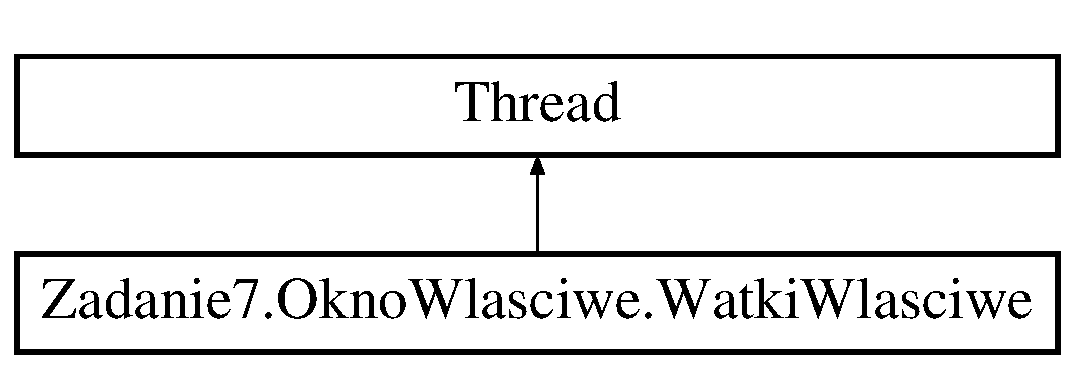
\includegraphics[height=2.000000cm]{class_zadanie7_1_1_okno_wlasciwe_1_1_watki_wlasciwe}
\end{center}
\end{figure}
\subsection*{Public Member Functions}
\begin{DoxyCompactItemize}
\item 
\hyperlink{class_zadanie7_1_1_okno_wlasciwe_1_1_watki_wlasciwe_a1115b2ad5f88ed9e0b3435a5bbc7d60a}{Watki\+Wlasciwe} (int \hyperlink{class_zadanie7_1_1_okno_wlasciwe_1_1_watki_wlasciwe_a28c612e4cd60226257222d9070a2e9f7}{i1}, int \hyperlink{class_zadanie7_1_1_okno_wlasciwe_1_1_watki_wlasciwe_a786ddbb34c817fbc00f1b46dc931f225}{j1}, Color\mbox{[}$\,$\mbox{]}\mbox{[}$\,$\mbox{]} \hyperlink{class_zadanie7_1_1_okno_wlasciwe_1_1_watki_wlasciwe_a49a3e6dd42f69b24a442855b7407e51e}{kolor}, Rectangle2D\mbox{[}$\,$\mbox{]}\mbox{[}$\,$\mbox{]} \hyperlink{class_zadanie7_1_1_okno_wlasciwe_1_1_watki_wlasciwe_ac3435b7920d2703e6dac78ec74ac36d6}{t}, int \hyperlink{class_zadanie7_1_1_okno_wlasciwe_1_1_watki_wlasciwe_a2e0f32af73eb52749d152f59e5278f45}{m}, int \hyperlink{class_zadanie7_1_1_okno_wlasciwe_1_1_watki_wlasciwe_a1e976e2b4da195c9013b64ed548cd0ca}{n}, int \hyperlink{class_zadanie7_1_1_okno_wlasciwe_1_1_watki_wlasciwe_a22e8786a26cf4b1898ae0d69f4bd01b9}{p}, int \hyperlink{class_zadanie7_1_1_okno_wlasciwe_1_1_watki_wlasciwe_a6a683092fcf7c93da165c5d0dc13ea01}{k})
\begin{DoxyCompactList}\small\item\em Tworzenie watku. \end{DoxyCompactList}\item 
void \hyperlink{class_zadanie7_1_1_okno_wlasciwe_1_1_watki_wlasciwe_af2c065d19491d613d38eea3727e9f8ca}{run} ()
\end{DoxyCompactItemize}
\subsection*{Package Attributes}
\begin{DoxyCompactItemize}
\item 
int \hyperlink{class_zadanie7_1_1_okno_wlasciwe_1_1_watki_wlasciwe_a786ddbb34c817fbc00f1b46dc931f225}{j1}
\item 
int \hyperlink{class_zadanie7_1_1_okno_wlasciwe_1_1_watki_wlasciwe_a22e8786a26cf4b1898ae0d69f4bd01b9}{p}
\item 
int \hyperlink{class_zadanie7_1_1_okno_wlasciwe_1_1_watki_wlasciwe_a6a683092fcf7c93da165c5d0dc13ea01}{k}
\item 
int \hyperlink{class_zadanie7_1_1_okno_wlasciwe_1_1_watki_wlasciwe_a2e0f32af73eb52749d152f59e5278f45}{m}
\item 
int \hyperlink{class_zadanie7_1_1_okno_wlasciwe_1_1_watki_wlasciwe_a1e976e2b4da195c9013b64ed548cd0ca}{n}
\end{DoxyCompactItemize}
\subsection*{Private Attributes}
\begin{DoxyCompactItemize}
\item 
int \hyperlink{class_zadanie7_1_1_okno_wlasciwe_1_1_watki_wlasciwe_a28c612e4cd60226257222d9070a2e9f7}{i1}
\item 
Color\mbox{[}$\,$\mbox{]}\mbox{[}$\,$\mbox{]} \hyperlink{class_zadanie7_1_1_okno_wlasciwe_1_1_watki_wlasciwe_a49a3e6dd42f69b24a442855b7407e51e}{kolor}
\item 
Rectangle2D\mbox{[}$\,$\mbox{]}\mbox{[}$\,$\mbox{]} \hyperlink{class_zadanie7_1_1_okno_wlasciwe_1_1_watki_wlasciwe_ac3435b7920d2703e6dac78ec74ac36d6}{t}
\item 
Lock \hyperlink{class_zadanie7_1_1_okno_wlasciwe_1_1_watki_wlasciwe_a346580729de0ff1e3afbad1301b8e4b1}{lock} = new Reentrant\+Lock()
\end{DoxyCompactItemize}


\subsection{Constructor \& Destructor Documentation}
\index{Zadanie7\+::\+Okno\+Wlasciwe\+::\+Watki\+Wlasciwe@{Zadanie7\+::\+Okno\+Wlasciwe\+::\+Watki\+Wlasciwe}!Watki\+Wlasciwe@{Watki\+Wlasciwe}}
\index{Watki\+Wlasciwe@{Watki\+Wlasciwe}!Zadanie7\+::\+Okno\+Wlasciwe\+::\+Watki\+Wlasciwe@{Zadanie7\+::\+Okno\+Wlasciwe\+::\+Watki\+Wlasciwe}}
\subsubsection[{\texorpdfstring{Watki\+Wlasciwe(int i1, int j1, Color[][] kolor, Rectangle2D[][] t, int m, int n, int p, int k)}{WatkiWlasciwe(int i1, int j1, Color[][] kolor, Rectangle2D[][] t, int m, int n, int p, int k)}}]{\setlength{\rightskip}{0pt plus 5cm}Zadanie7.\+Okno\+Wlasciwe.\+Watki\+Wlasciwe.\+Watki\+Wlasciwe (
\begin{DoxyParamCaption}
\item[{int}]{i1, }
\item[{int}]{j1, }
\item[{Color}]{kolor\mbox{[}$\,$\mbox{]}\mbox{[}$\,$\mbox{]}, }
\item[{Rectangle2D}]{t\mbox{[}$\,$\mbox{]}\mbox{[}$\,$\mbox{]}, }
\item[{int}]{m, }
\item[{int}]{n, }
\item[{int}]{p, }
\item[{int}]{k}
\end{DoxyParamCaption}
)}\hypertarget{class_zadanie7_1_1_okno_wlasciwe_1_1_watki_wlasciwe_a1115b2ad5f88ed9e0b3435a5bbc7d60a}{}\label{class_zadanie7_1_1_okno_wlasciwe_1_1_watki_wlasciwe_a1115b2ad5f88ed9e0b3435a5bbc7d60a}


Tworzenie watku. 


\begin{DoxyParams}{Parameters}
{\em i1,j1} & \char`\"{}wsporzedne\char`\"{} naszego watku w tablicy (int) \\
\hline
{\em kolor} & tablica kolorow na ktorej watek bedzie pracowac (Color\mbox{[}\mbox{]}\mbox{[}\mbox{]}) \\
\hline
{\em t} & tablica \char`\"{}boksow\char`\"{} ktorzy kolory beda zmieniane w czasie prezentacji (Rectangle2D\mbox{[}\mbox{]}\mbox{[}\mbox{]}) \\
\hline
{\em m} & szerokosc planszy liczona w boksach (int) \\
\hline
{\em n} & wysokosc planszy liczona w boksach (int) \\
\hline
{\em k} & szybkosc dzialania programu, im wiecej tym wolniej (int) \\
\hline
{\em p} & prawdopodobienstwo w procentach (int) \\
\hline
\end{DoxyParams}


\subsection{Member Function Documentation}
\index{Zadanie7\+::\+Okno\+Wlasciwe\+::\+Watki\+Wlasciwe@{Zadanie7\+::\+Okno\+Wlasciwe\+::\+Watki\+Wlasciwe}!run@{run}}
\index{run@{run}!Zadanie7\+::\+Okno\+Wlasciwe\+::\+Watki\+Wlasciwe@{Zadanie7\+::\+Okno\+Wlasciwe\+::\+Watki\+Wlasciwe}}
\subsubsection[{\texorpdfstring{run()}{run()}}]{\setlength{\rightskip}{0pt plus 5cm}void Zadanie7.\+Okno\+Wlasciwe.\+Watki\+Wlasciwe.\+run (
\begin{DoxyParamCaption}
{}
\end{DoxyParamCaption}
)}\hypertarget{class_zadanie7_1_1_okno_wlasciwe_1_1_watki_wlasciwe_af2c065d19491d613d38eea3727e9f8ca}{}\label{class_zadanie7_1_1_okno_wlasciwe_1_1_watki_wlasciwe_af2c065d19491d613d38eea3727e9f8ca}


\subsection{Member Data Documentation}
\index{Zadanie7\+::\+Okno\+Wlasciwe\+::\+Watki\+Wlasciwe@{Zadanie7\+::\+Okno\+Wlasciwe\+::\+Watki\+Wlasciwe}!i1@{i1}}
\index{i1@{i1}!Zadanie7\+::\+Okno\+Wlasciwe\+::\+Watki\+Wlasciwe@{Zadanie7\+::\+Okno\+Wlasciwe\+::\+Watki\+Wlasciwe}}
\subsubsection[{\texorpdfstring{i1}{i1}}]{\setlength{\rightskip}{0pt plus 5cm}int Zadanie7.\+Okno\+Wlasciwe.\+Watki\+Wlasciwe.\+i1\hspace{0.3cm}{\ttfamily [private]}}\hypertarget{class_zadanie7_1_1_okno_wlasciwe_1_1_watki_wlasciwe_a28c612e4cd60226257222d9070a2e9f7}{}\label{class_zadanie7_1_1_okno_wlasciwe_1_1_watki_wlasciwe_a28c612e4cd60226257222d9070a2e9f7}
\index{Zadanie7\+::\+Okno\+Wlasciwe\+::\+Watki\+Wlasciwe@{Zadanie7\+::\+Okno\+Wlasciwe\+::\+Watki\+Wlasciwe}!j1@{j1}}
\index{j1@{j1}!Zadanie7\+::\+Okno\+Wlasciwe\+::\+Watki\+Wlasciwe@{Zadanie7\+::\+Okno\+Wlasciwe\+::\+Watki\+Wlasciwe}}
\subsubsection[{\texorpdfstring{j1}{j1}}]{\setlength{\rightskip}{0pt plus 5cm}int Zadanie7.\+Okno\+Wlasciwe.\+Watki\+Wlasciwe.\+j1\hspace{0.3cm}{\ttfamily [package]}}\hypertarget{class_zadanie7_1_1_okno_wlasciwe_1_1_watki_wlasciwe_a786ddbb34c817fbc00f1b46dc931f225}{}\label{class_zadanie7_1_1_okno_wlasciwe_1_1_watki_wlasciwe_a786ddbb34c817fbc00f1b46dc931f225}
\index{Zadanie7\+::\+Okno\+Wlasciwe\+::\+Watki\+Wlasciwe@{Zadanie7\+::\+Okno\+Wlasciwe\+::\+Watki\+Wlasciwe}!k@{k}}
\index{k@{k}!Zadanie7\+::\+Okno\+Wlasciwe\+::\+Watki\+Wlasciwe@{Zadanie7\+::\+Okno\+Wlasciwe\+::\+Watki\+Wlasciwe}}
\subsubsection[{\texorpdfstring{k}{k}}]{\setlength{\rightskip}{0pt plus 5cm}int Zadanie7.\+Okno\+Wlasciwe.\+Watki\+Wlasciwe.\+k\hspace{0.3cm}{\ttfamily [package]}}\hypertarget{class_zadanie7_1_1_okno_wlasciwe_1_1_watki_wlasciwe_a6a683092fcf7c93da165c5d0dc13ea01}{}\label{class_zadanie7_1_1_okno_wlasciwe_1_1_watki_wlasciwe_a6a683092fcf7c93da165c5d0dc13ea01}
\index{Zadanie7\+::\+Okno\+Wlasciwe\+::\+Watki\+Wlasciwe@{Zadanie7\+::\+Okno\+Wlasciwe\+::\+Watki\+Wlasciwe}!kolor@{kolor}}
\index{kolor@{kolor}!Zadanie7\+::\+Okno\+Wlasciwe\+::\+Watki\+Wlasciwe@{Zadanie7\+::\+Okno\+Wlasciwe\+::\+Watki\+Wlasciwe}}
\subsubsection[{\texorpdfstring{kolor}{kolor}}]{\setlength{\rightskip}{0pt plus 5cm}Color \mbox{[}$\,$\mbox{]}\mbox{[}$\,$\mbox{]} Zadanie7.\+Okno\+Wlasciwe.\+Watki\+Wlasciwe.\+kolor\hspace{0.3cm}{\ttfamily [private]}}\hypertarget{class_zadanie7_1_1_okno_wlasciwe_1_1_watki_wlasciwe_a49a3e6dd42f69b24a442855b7407e51e}{}\label{class_zadanie7_1_1_okno_wlasciwe_1_1_watki_wlasciwe_a49a3e6dd42f69b24a442855b7407e51e}
\index{Zadanie7\+::\+Okno\+Wlasciwe\+::\+Watki\+Wlasciwe@{Zadanie7\+::\+Okno\+Wlasciwe\+::\+Watki\+Wlasciwe}!lock@{lock}}
\index{lock@{lock}!Zadanie7\+::\+Okno\+Wlasciwe\+::\+Watki\+Wlasciwe@{Zadanie7\+::\+Okno\+Wlasciwe\+::\+Watki\+Wlasciwe}}
\subsubsection[{\texorpdfstring{lock}{lock}}]{\setlength{\rightskip}{0pt plus 5cm}Lock Zadanie7.\+Okno\+Wlasciwe.\+Watki\+Wlasciwe.\+lock = new Reentrant\+Lock()\hspace{0.3cm}{\ttfamily [private]}}\hypertarget{class_zadanie7_1_1_okno_wlasciwe_1_1_watki_wlasciwe_a346580729de0ff1e3afbad1301b8e4b1}{}\label{class_zadanie7_1_1_okno_wlasciwe_1_1_watki_wlasciwe_a346580729de0ff1e3afbad1301b8e4b1}
\index{Zadanie7\+::\+Okno\+Wlasciwe\+::\+Watki\+Wlasciwe@{Zadanie7\+::\+Okno\+Wlasciwe\+::\+Watki\+Wlasciwe}!m@{m}}
\index{m@{m}!Zadanie7\+::\+Okno\+Wlasciwe\+::\+Watki\+Wlasciwe@{Zadanie7\+::\+Okno\+Wlasciwe\+::\+Watki\+Wlasciwe}}
\subsubsection[{\texorpdfstring{m}{m}}]{\setlength{\rightskip}{0pt plus 5cm}int Zadanie7.\+Okno\+Wlasciwe.\+Watki\+Wlasciwe.\+m\hspace{0.3cm}{\ttfamily [package]}}\hypertarget{class_zadanie7_1_1_okno_wlasciwe_1_1_watki_wlasciwe_a2e0f32af73eb52749d152f59e5278f45}{}\label{class_zadanie7_1_1_okno_wlasciwe_1_1_watki_wlasciwe_a2e0f32af73eb52749d152f59e5278f45}
\index{Zadanie7\+::\+Okno\+Wlasciwe\+::\+Watki\+Wlasciwe@{Zadanie7\+::\+Okno\+Wlasciwe\+::\+Watki\+Wlasciwe}!n@{n}}
\index{n@{n}!Zadanie7\+::\+Okno\+Wlasciwe\+::\+Watki\+Wlasciwe@{Zadanie7\+::\+Okno\+Wlasciwe\+::\+Watki\+Wlasciwe}}
\subsubsection[{\texorpdfstring{n}{n}}]{\setlength{\rightskip}{0pt plus 5cm}int Zadanie7.\+Okno\+Wlasciwe.\+Watki\+Wlasciwe.\+n\hspace{0.3cm}{\ttfamily [package]}}\hypertarget{class_zadanie7_1_1_okno_wlasciwe_1_1_watki_wlasciwe_a1e976e2b4da195c9013b64ed548cd0ca}{}\label{class_zadanie7_1_1_okno_wlasciwe_1_1_watki_wlasciwe_a1e976e2b4da195c9013b64ed548cd0ca}
\index{Zadanie7\+::\+Okno\+Wlasciwe\+::\+Watki\+Wlasciwe@{Zadanie7\+::\+Okno\+Wlasciwe\+::\+Watki\+Wlasciwe}!p@{p}}
\index{p@{p}!Zadanie7\+::\+Okno\+Wlasciwe\+::\+Watki\+Wlasciwe@{Zadanie7\+::\+Okno\+Wlasciwe\+::\+Watki\+Wlasciwe}}
\subsubsection[{\texorpdfstring{p}{p}}]{\setlength{\rightskip}{0pt plus 5cm}int Zadanie7.\+Okno\+Wlasciwe.\+Watki\+Wlasciwe.\+p\hspace{0.3cm}{\ttfamily [package]}}\hypertarget{class_zadanie7_1_1_okno_wlasciwe_1_1_watki_wlasciwe_a22e8786a26cf4b1898ae0d69f4bd01b9}{}\label{class_zadanie7_1_1_okno_wlasciwe_1_1_watki_wlasciwe_a22e8786a26cf4b1898ae0d69f4bd01b9}
\index{Zadanie7\+::\+Okno\+Wlasciwe\+::\+Watki\+Wlasciwe@{Zadanie7\+::\+Okno\+Wlasciwe\+::\+Watki\+Wlasciwe}!t@{t}}
\index{t@{t}!Zadanie7\+::\+Okno\+Wlasciwe\+::\+Watki\+Wlasciwe@{Zadanie7\+::\+Okno\+Wlasciwe\+::\+Watki\+Wlasciwe}}
\subsubsection[{\texorpdfstring{t}{t}}]{\setlength{\rightskip}{0pt plus 5cm}Rectangle2D \mbox{[}$\,$\mbox{]}\mbox{[}$\,$\mbox{]} Zadanie7.\+Okno\+Wlasciwe.\+Watki\+Wlasciwe.\+t\hspace{0.3cm}{\ttfamily [private]}}\hypertarget{class_zadanie7_1_1_okno_wlasciwe_1_1_watki_wlasciwe_ac3435b7920d2703e6dac78ec74ac36d6}{}\label{class_zadanie7_1_1_okno_wlasciwe_1_1_watki_wlasciwe_ac3435b7920d2703e6dac78ec74ac36d6}


The documentation for this class was generated from the following file\+:\begin{DoxyCompactItemize}
\item 
\hyperlink{_okno_wlasciwe_8java}{Okno\+Wlasciwe.\+java}\end{DoxyCompactItemize}

\chapter{File Documentation}
\hypertarget{_main_8java}{}\section{Main.\+java File Reference}
\label{_main_8java}\index{Main.\+java@{Main.\+java}}
\subsection*{Classes}
\begin{DoxyCompactItemize}
\item 
class \hyperlink{class_zadanie7_1_1_main}{Zadanie7.\+Main}
\end{DoxyCompactItemize}
\subsection*{Packages}
\begin{DoxyCompactItemize}
\item 
package \hyperlink{namespace_zadanie7}{Zadanie7}
\end{DoxyCompactItemize}

\hypertarget{_okno_pierwsze_8java}{}\section{Okno\+Pierwsze.\+java File Reference}
\label{_okno_pierwsze_8java}\index{Okno\+Pierwsze.\+java@{Okno\+Pierwsze.\+java}}
\subsection*{Classes}
\begin{DoxyCompactItemize}
\item 
class \hyperlink{class_zadanie7_1_1_okno_pierwsze}{Zadanie7.\+Okno\+Pierwsze}
\end{DoxyCompactItemize}
\subsection*{Packages}
\begin{DoxyCompactItemize}
\item 
package \hyperlink{namespace_zadanie7}{Zadanie7}
\end{DoxyCompactItemize}

\hypertarget{_okno_wlasciwe_8java}{}\section{Okno\+Wlasciwe.\+java File Reference}
\label{_okno_wlasciwe_8java}\index{Okno\+Wlasciwe.\+java@{Okno\+Wlasciwe.\+java}}
\subsection*{Classes}
\begin{DoxyCompactItemize}
\item 
class \hyperlink{class_zadanie7_1_1_okno_wlasciwe}{Zadanie7.\+Okno\+Wlasciwe}
\item 
class \hyperlink{class_zadanie7_1_1_okno_wlasciwe_1_1_watki_wlasciwe}{Zadanie7.\+Okno\+Wlasciwe.\+Watki\+Wlasciwe}
\end{DoxyCompactItemize}
\subsection*{Packages}
\begin{DoxyCompactItemize}
\item 
package \hyperlink{namespace_zadanie7}{Zadanie7}
\end{DoxyCompactItemize}

%--- End generated contents ---

% Index
\backmatter
\newpage
\phantomsection
\clearemptydoublepage
\addcontentsline{toc}{chapter}{Index}
\printindex

\end{document}
